%%
%% This is file `sample-acmsmall.tex',
%% generated with the docstrip utility.
%%
%% The original source files were:
%%
%% samples.dtx  (with options: `acmsmall')
%% 
%% IMPORTANT NOTICE:
%% 
%% For the copyright see the source file.
%% 
%% Any modified versions of this file must be renamed
%% with new filenames distinct from sample-acmsmall.tex.
%% 
%% For distribution of the original source see the terms
%% for copying and modification in the file samples.dtx.
%% 
%% This generated file may be distributed as long as the
%% original source files, as listed above, are part of the
%% same distribution. (The sources need not necessarily be
%% in the same archive or directory.)
%%
%%
%% Commands for TeXCount
%TC:macro \cite [option:text,text]
%TC:macro \citep [option:text,text]
%TC:macro \citet [option:text,text]
%TC:envir table 0 1
%TC:envir table* 0 1
%TC:envir tabular [ignore] word
%TC:envir displaymath 0 word
%TC:envir math 0 word
%TC:envir comment 0 0
%%
%%
%% The first command in your LaTeX source must be the \documentclass
%% command.
%%
%% For submission and review of your manuscript please change the
%% command to \documentclass[manuscript, screen, review]{acmart}.
%%
%% When submitting camera ready or to TAPS, please change the command
%% to \documentclass[sigconf]{acmart} or whichever template is required
%% for your publication.
%%
%%
\documentclass[acmsmall]{acmart}
\usepackage{mathpartir}
\newcommand{\name}{\text{Zombie}\xspace}

\newcommand{\sLet}{\text{\textsf{Let}}\xspace}
\newcommand{\sLam}{\text{\textsf{Lam}}\xspace}
\newcommand{\sApp}{\text{\textsf{App}}\xspace}
\newcommand{\sProd}{\text{\textsf{Prod}}\xspace}
\newcommand{\sZro}{\text{\textsf{Zro}}\xspace}
\newcommand{\sFst}{\text{\textsf{Fst}}\xspace}
\newcommand{\sLeft}{\text{\textsf{Left}}\xspace}
\newcommand{\sRight}{\text{\textsf{Right}}\xspace}
\newcommand{\sCase}{\text{\textsf{Case}}\xspace}
\newcommand{\sIn}{\text{\textsf{in}}\xspace}
\newcommand{\sOf}{\text{\textsf{of}}\xspace}

\newcommand{\Env}{\ensuremath{E}\xspace}
\newcommand{\KCell}{\text{\textnormal{KCell}}\xspace}
\newcommand{\VCell}{\text{\textnormal{VCell}}\xspace}
\newcommand{\KLet}{\text{\textsf{KLet}}\xspace}
\newcommand{\KLookup}{\text{\textsf{KLookup}}\xspace}
\newcommand{\Done}{\text{\textsf{Done}}\xspace}
\newcommand{\KApp}{\text{\textsf{KApp}}\xspace}
\newcommand{\KProd}{\text{\textsf{KProd}}\xspace}
\newcommand{\KZro}{\text{\textsf{KZro}}\xspace}
\newcommand{\KFst}{\text{\textsf{KFst}}\xspace}
\newcommand{\KLeft}{\text{\textsf{KLeft}}\xspace}
\newcommand{\KRight}{\text{\textsf{KRight}}\xspace}
\newcommand{\KCase}{\text{\textsf{KCase}}\xspace}
\newcommand{\Clos}{\text{\textsf{Clos}}\xspace}
\newcommand{\VProd}{\text{\textsf{VProd}}\xspace}
\newcommand{\VLeft}{\text{\textsf{VLeft}}\xspace}
\newcommand{\VRight}{\text{\textsf{VRight}}\xspace}
\newcommand{\Eval}{\text{\textsf{Eval}}\xspace}
\newcommand{\Apply}{\text{\textsf{Apply}}\xspace}

\newcommand{\RKApply}{\text{\textsf{RKApply}}\xspace}
\newcommand{\RHApply}{\text{\textsf{RHApply}}\xspace}
\newcommand{\RHCase}{\text{\textsf{RHCase}}\xspace}
\newcommand{\RHZro}{\text{\textsf{RHZro}}\xspace}
\newcommand{\RHFst}{\text{\textsf{RHFst}}\xspace}
\newcommand{\RHApp}{\text{\textsf{RHApp}}\xspace}
\newcommand{\RApply}{\text{\textsf{RApply}}\xspace}

\newcommand{\Just}{\textrm{Just}}
\newcommand{\Nothing}{\textrm{Nothing}}

\newcommand{\Alloc}{\textrm{Alloc}}
\newcommand{\Lookup}{\textrm{Lookup}}

\newcommand{\Insert}{\text{\textsf{Insert}}\xspace}

\newcommand{\NoReplay}{\text{\textsf{NoReplay}}\xspace}
\newcommand{\Replaying}{\text{\textsf{Replaying}}\xspace}


%%
%% \BibTeX command to typeset BibTeX logo in the docs
\AtBeginDocument{%
	\providecommand\BibTeX{{%
			Bib\TeX}}}

%% Rights management information.  This information is sent to you
%% when you complete the rights form.  These commands have SAMPLE
%% values in them; it is your responsibility as an author to replace
%% the commands and values with those provided to you when you
%% complete the rights form.
\setcopyright{acmlicensed}
\copyrightyear{2018}
\acmYear{2018}
\acmDOI{XXXXXXX.XXXXXXX}


%%
%% These commands are for a JOURNAL article.
\acmJournal{JACM}
\acmVolume{37}
\acmNumber{4}
\acmArticle{111}
\acmMonth{8}

%%
%% Submission ID.
%% Use this when submitting an article to a sponsored event. You'll
%% receive a unique submission ID from the organizers
%% of the event, and this ID should be used as the parameter to this command.
%%\acmSubmissionID{123-A56-BU3}

%%
%% For managing citations, it is recommended to use bibliography
%% files in BibTeX format.
%%
%% You can then either use BibTeX with the ACM-Reference-Format style,
%% or BibLaTeX with the acmnumeric or acmauthoryear sytles, that include
%% support for advanced citation of software artefact from the
%% biblatex-software package, also separately available on CTAN.
%%
%% Look at the sample-*-biblatex.tex files for templates showcasing
%% the biblatex styles.
%%

%%
%% The majority of ACM publications use numbered citations and
%% references.  The command \citestyle{authoryear} switches to the
%% "author year" style.
%%
%% If you are preparing content for an event
%% sponsored by ACM SIGGRAPH, you must use the "author year" style of
%% citations and references.
%% Uncommenting
%% the next command will enable that style.
%%\citestyle{acmauthoryear}

\usepackage{xcolor}
\usepackage{mdframed}
\newcommand\todo[1]{\textcolor{red}{#1}}
\newcommand\pavel{\todo{pavel look here} }

%%
%% end of the preamble, start of the body of the document source.
\begin{document}
	%%
	%% The "title" command has an optional parameter,
	%% allowing the author to define a "short title" to be used in page headers.
	\title{Uncomputation}
	%%
	%% The "author" command and its associated commands are used to define
	%% the authors and their affiliations.
	%% Of note is the shared affiliation of the first two authors, and the
	%% "authornote" and "authornotemark" commands
	%% used to denote shared contribution to the research.
	\author{Maisa Kirisame}
	\email{marisa@cs.utah.edu}
	\orcid{1234-5678-9012}
	\authornotemark[1]
	\affiliation{%
		\institution{University of Utah}
		\streetaddress{P.O. Box 1212}
		\city{Salt Lake City}
		\state{Utah}
		\country{USA}
		\postcode{43017-6221}
	}

	\author{Pavel Panchekha}
	\email{}
	\orcid{1234-5678-9012}
	\authornotemark[1]
	\affiliation{%
		\institution{University of Utah}
		\streetaddress{P.O. Box 1212}
		\city{Salt Lake City}
		\state{Utah}
		\country{USA}
		\postcode{43017-6221}
	}
	
	%%
	%% By default, the full list of authors will be used in the page
	%% headers. Often, this list is too long, and will overlap
	%% other information printed in the page headers. This command allows
	%% the author to define a more concise list
	%% of authors' names for this purpose.
	\renewcommand{\shortauthors}{Kirisame et al.}
	%%
	%% The abstract is a short summary of the work to be presented in the
	%% article.
	\begin{abstract}
		Program execution need memory. Program may run out of memory for multiple reasons: big dataset, exploding intermediate state, the machine have less memory than others, etc. When this happens, the program either get killed, or the operating system swaps, significantly degrading the performance.
		We propose a technique, uncomputation, that allow the program to continue running gracefully even after breaching the memory limit, without significant performance degradation.
		Uncomputation work by turning computed values back into thunk, and upon re-requesting the thunk, computing and storing them back.
		A naive implementation of uncomputation will face multiple problems. Among them, the most crucial and the most challenging one is that of breadcrumb. After a value is uncomputed, it's memory can be released but some memory, breadcrumb, is needed, so we can recompute the value back.
		Ironically, in a applicative language, due to boxing all values are small. This mean uncomputation, implemented naively, will only consume more memory, defeating the purpose.
		We present a runtime system, implemented as a library, that is absolved of the above breadcrumb problem, seemingly storing recompute information in 0-bits and violating information theory.
	\end{abstract}
	
	%%
	%% The code below is generated by the tool at http://dl.acm.org/ccs.cfm.
	%% Please copy and paste the code instead of the example below.
	%%
		
	%%
	%% Keywords. The author(s) should pick words that accurately describe
	%% the work being presented. Separate the keywords with commas.
	\keywords{Do, Not, Us, This, Code, Put, the, Correct, Terms, for,
		Your, Paper}
	
	\received{20 February 2007}
	\received[revised]{12 March 2009}
	\received[accepted]{5 June 2009}
	
	%%
	%% This command processes the author and affiliation and title
	%% information and builds the first part of the formatted document.
	\maketitle
	\section{Intro}
	\section{Overview}	
	FIGURE draw attention to KEY IDEA

explain argument
key steps
dependency between steps
focus on the dependency

Section: CEK Machine: pointers, lookup, allocate substeps (2.5-3pg long)
Figure: draw on whiteboard, take screenshot.

Section: Tocks (5pg long)
tock: exploit linear property of CEK machine
talk about time instead of memory
mapping stored in an ordered tree
Context (not a section)
map is sparse
lookup fail, need to recompute
also store CEK context

Section: The CEKR Machine (???)
Replay Stack
the section with lots of greeks
argue about progress

Section: Implementation (3pg long)
Heuristic
Loop Unrolling

Key question: How to get the replay stack small?
Key question: Garbage Collection/Eager Eviction

Summarize the meeting into key step

Sad Path

Replay Stack

Double O(1)

Quality


Another kind of thing in tock tree.

Transition from X -> Y

Allocated during the transition

Map from tock to Cell | Context

	\section{Core Language}	

Zombie works on a purely functional language with products, sum types,
and first-class functions called $\lambda_Z$. For simplicity in this
paper, we treat the language as untyped. The syntax of $\lambda_Z$ is
shown in \Cref{fig:syntax}; its semantics are standard. The full
Zombie implementation supports additional features, such as primitive
types and input/output; \Cref{sec:impl} describes how these features
are layered on top of the core implementation described here.

Importantly, because Zombie is purely functional, programs are totally
deterministic, in the sense that evaluating a given expression in a
given environment always returns the same result. This is essential
for Zombie to work correctly.

\subsection{CEK Machine}

The key insight of Zombie is to assign an unique identifier to any
value ever allocated during the program's execution. Conceptually, it
identifies each value with the execution step that allocated it. It
does this using a variant of the CEK machine.

The CEK machine is a well-known abstract machine for executing untyped
lambda calculi, where the machine state consists of three parts:

\begin{enumerate}
	\item \textcolor{blue}{C}ontrol, the expression currently being evaluated.
	\item \textcolor{blue}{E}nvironment,
          a map from the free variables of the Control to their values.
	\item \textcolor{blue}{K}ontinuation, which is to be invoked
          with the value the Control evaluates to.
\end{enumerate}

\todo{We should use $C$ for expressions, to match the CEK terminology.}

In our variation of the CEK machine, we split the evaluation phase
from the invocation of the continuation, resulting in a machine state
that looks like this:
\[
\text{State} \operatorname{::=} \Eval~E~\Env~K \mid \Apply~K~V
\]
In other words, our CEK machine can be in an $\Eval$ or an $\Apply$
state; the $\Eval$ stores the classic control, environment, and
kontinuation, while the $\Apply$ state stores just a continuation and
a value. The precise syntax of values and kontinuations are given in
\Cref{fig:defs}.

Execution in the CEK machine involves a series of transitions between
these machine states; in other words, it is a transition system. To
run a program $C$ in the CEK machine, one first sets up an initial
state $(\Eval~C~\{\}~\Done)$ whose Control is the expression to
evaluate, whose Environment is empty, and whose Kontinuation is a
special $\Done$ continuation. The rules of the CEK machine are then
used to transition from one machine state to another, until finally
reaching the state $\Apply~\Done~V$. In that state, $V$ is the result
of evaluating of $C$.%
\footnote{Note that, because $\lambda_Z$ is untyped, it contains
non-terminating programs using, for example, the $Y$ combinator. In
the CEK machine, these programs create an infinite sequence of machine
states that do not include a terminating $\Apply~\Done~V$.}

A notable property of the CEK machine is that each transition performs
a bounded amount of work. Contrast this to a traditional operation
semantics, where the semantics of a \sCase statement might be something
like:

\begin{mathpar}
 \inferrule{
   \Gamma \vdash e \to^* \sLeft~\Gamma' \vdash V
 }{\Gamma \vdash \sCase~e~x~e_l~y~e_r
   \to \Gamma', x : V \vdash e_l
 }
\end{mathpar}

Here the antecedent of the inference rule might perform arbitrarily
many steps, and thus an arbitrary amount of computation; derivations
thus form a tree. In the CEK machine, no such steps exist, and
derivations in the CEK machine form a flat list. This property of the
CEK machine is illustrated graphically in \Cref{fig:constant}.

\begin{figure}
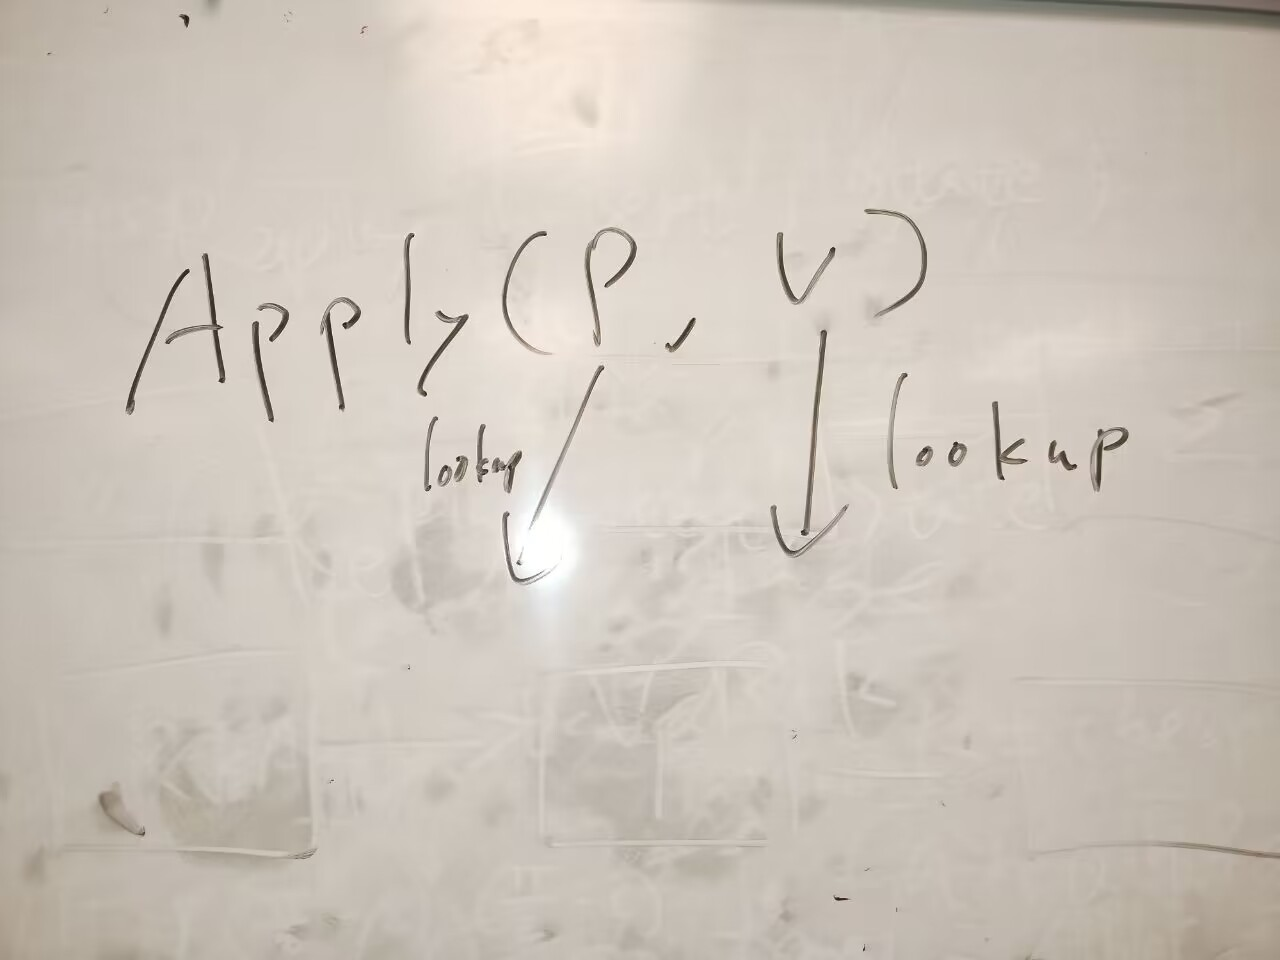
\includegraphics[width=0.5\columnwidth]{1}
\caption{the machine does a small constant amount of pointer lookup}
\label{fig:constant}
\end{figure}

\subsection{Determinism and Tocks}

Importantly, the CEK machine is linear and deterministic. This means
that every CEK machine state transitions to at most one state. That in
turn means that if we were to ``rewind'' a CEK machine, putting it in
an earlier state, it would transition through the exact same sequence
of states in the exact same order. This determinism or
``replayability'' is essential for Zombie to work, and is illustrated
graphically in \Cref{fig:replayability}.

\begin{figure}
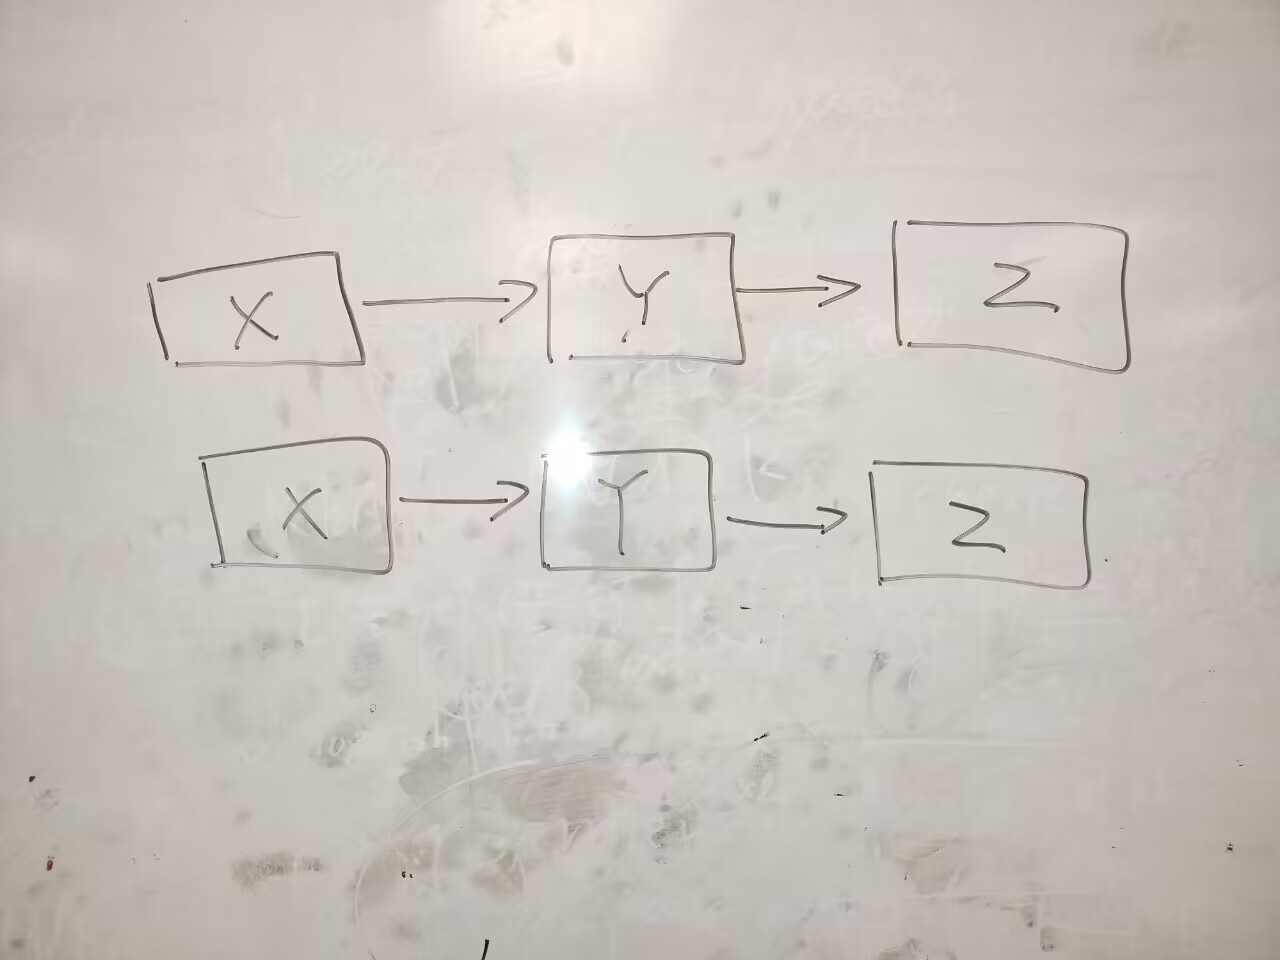
\includegraphics[width=0.5\columnwidth]{0}
\caption{the deterministic, linear nature of the CEK machine}
\label{fig:replayability}
\end{figure}

One key property guaranteed by determinism is that, for a given
initial program $C$, the machine state at any point during $C$'s
execution can be uniquely identified by how many steps have been
executed since the initial state. In other words, the initial state is
identified with the number $0$, the next state it transitions to with
the number $1$, and so on. This state number, which we call a
``tock'', is logically unbounded, but in our implementation it is
stored as a 64-bit integer. In our implementation, that suffices for
several decades of runtime on current hardware. 

\subsection{Heap Memory}

Because we are interested the total memory usage of $\lambda_Z$
program, our variant of the CEK machine includes an explicit heap and
explicit pointers. That is, in our formalization values $V$ are
formalized as pointers $P\langle \VCell \rangle$ to ``value cells''.
Values cells---which can be closures, products, and sums---in turn
contain values, that is, pointers.

During execution, the CEK machine looks up these values using an
explicit heap $H$. To interact with the heap, the CEK machine uses two
functions. $\Lookup : (P \langle X \rangle, H) \to X$ dereferences a
pointer in the heap. $\Alloc : (X, H) \to (P \langle X \rangle, H')$
stores a value in the heap, returning a pointer to it and the updated
heap. Transitions in the CEK machine call $\Lookup$ and $\Alloc$ in
order to make $\Eval$ and $\Apply$ steps, as shown in \Cref{fig:eval}
and \Cref{fig:apply}.

Importantly, every CEK machine step (whether $\Eval$ or $\Apply$)
makes at most one call to $\Lookup$ and at most one call to $\Alloc$. 
This means that each allocation the program
makes can be uniquely identified by the tock for the machine state
where it is allocated. This identification is the core abstraction
that drives Zombie's implementation.

\newcommand{\mytableshape}{p{6em} p{2.6em} p{1em} p{0.45\textwidth}}
\begin{figure}
	\begin{tabular}{\mytableshape}
		Name & $N$ & $::=$ & A set of distinct names \\
		Expr & $E$ & $::=$ & $
		N \mid
		\sLet~x=A~\sIn~B \mid
		\backslash x.~A \mid
		f(x) \mid
		(x, y) \mid
		x.0 \mid
		x.1 \mid
		\sLeft~x \mid
		\sRight~y \mid
		\sCase~x~\sOf~\sLeft~a\Rightarrow L~||~\sRight~b\Rightarrow R $
	\end{tabular}
	\caption{The syntax of $\lambda_Z$.}
        \label{fig:syntax}
\end{figure}

\begin{figure}
	\begin{tabular}{\mytableshape}
		Heap & $H$ & $::=$ & An abstract key value store \\
		Pointer$\langle X \rangle$ & $P\langle X \rangle$ & $::=$ & Key into heap with value type $X$ \\
		Lookup & & : & $(\text{Pointer}\langle X \rangle, H) \to X$ \\
		Alloc & & : & $(X, H) \to (\text{Pointer}\langle X \rangle, H)$ \\
	\end{tabular}
	\caption{Heap API}
	\label{fig:heap}
\end{figure}

\begin{figure}
	\begin{tabular}{\mytableshape}
		Continuation & $K$ & $::=$ & $P \langle \KCell \rangle$ \\
		
		KCell & & $::=$ & $
		\Done \mid
		KLookup~K~ \mid
		\KLet~N~\Env~E~K \mid
		\KApp_0~\Env~E~K \mid
		\KApp_1~\Env~N~E~K \mid
		\KProd_0~\Env~E~K \mid
		\KProd_1~V~K \mid
		\KZro~K \mid
		\KFst~K \mid
		\KLeft~K \mid
		\KRight~K \mid
		\KCase~\Env~N~E~N~E~K $ \\
		
		Value & $V$ & $::=$ & $P\langle \VCell \rangle$ \\
		VCell & & $::=$ & $
		\Clos~\Env~N~E \mid
		\VProd~V~V \mid
		\VLeft~V \mid
		\VRight~V $ \\
		
		Environment & $\Env$ & ::= & $[(N, V)]$ \\
		State & & ::= & $\Eval~E~\Env~K \mid \Apply~KCell~V $ \\
	\end{tabular}
	\caption{Definitions for the CEK Machine}
        \label{fig:defs}
\end{figure}
\begin{figure}
	\begin{mathpar}
		\inferrule{ }{\text{State} \leadsto \text{State}} \and
		\inferrule{ }{\Eval(N, \Env, K) \leadsto \Apply(K, \Env(N))} \and
		\inferrule{ }{\Eval(\sLet~A=B~\sIn~C, \Env, K) \leadsto \Eval(B, \Env, \KLet~A~K~C~\Env)} \and
		\inferrule{ }{\Apply(\KLet~A~\Env~C~K, V) \leadsto \Eval(C, \Env[A := V], K)} \and
		\inferrule{ }{\Eval(\backslash N. E, \Env, K) \leadsto \Apply(K, \Clos~\Env(\text{fv})\cdots N~E)} \and
		\inferrule{ }{\Eval(F(X), \Env, K) \leadsto \Eval(F, \KApp_0~K~X)} \and
		\inferrule{ }{\Apply(\KApp_0~\Env~X~K, \Clos~\Env'~N~E) \leadsto \Eval(X, \Env, \KApp_1~\Env'~N~E~K)} \and
		\inferrule{ }{\Apply(\KApp_1~\Env~N~E~K, V) \leadsto \Eval(E, \Env[N := V], K)}
		\inferrule{ }{\Eval((L, R), \Env, K) \leadsto \Eval(L, \Env, \KProd_0~K~R)} \and
		\inferrule{ }{\Apply(\text{KProd0}~\Env~R~K, V) \leadsto \Eval(R, Env, \KProd_1~V~K)} \and
		\inferrule{ }{\Apply(\KProd_1~L~K, V) \leadsto \Apply(K, \VProd~L~V)} \and
		\inferrule{ }{\Eval(X.0, \Env, K) \leadsto \Eval(X, \Env, \KZro~K)} \and
		\inferrule{ }{\Apply(\KZro~K, \VProd~X~Y) \leadsto \Apply(K, X)} \and
		\inferrule{ }{\Eval(X.1, \Env, K) \leadsto \Eval(X, \Env, \KFst~K)} \and
		\inferrule{ }{\Apply(\KFst~K, \VProd~X~Y) \leadsto \Apply(K, Y)} \and
		\inferrule{ }{\Eval(\sLeft~X, \Env, K) \leadsto \Eval(X, \Env, \KLeft~K)} \and
		\inferrule{ }{\Apply(\KLeft~K, V) \leadsto \Apply(K, \VLeft~V)} \and
		\inferrule{ }{\Eval(\sRight~X, \Env, K) \leadsto \Eval(X, \Env, \KRight~K)} \and
		\inferrule{ }{\Apply(\KRight~K, V) \leadsto \Apply(K, \VRight~V)} \and
		\inferrule{ }{\Eval(\sCase~X~\sOf~\sLeft~LN\Rightarrow L~||~\sRight~RN\Rightarrow R, \Env, K) \leadsto \Eval(X, \Env, \KCase~\mathit{LN}~L~\mathit{RN}~R~\Env)} \and
		\inferrule{ }{\Apply(\KCase~\Env~\mathit{LN}~L~\mathit{RN}~R~K, VLeft V) \leadsto \Eval(L, \Env[\mathit{LN} := V], K)} \and
		\inferrule{ }{\Apply(\KCase~\Env~\mathit{LN}~L~\mathit{RN}~R~K, VRight V) \leadsto \Eval(R, \Env[\mathit{RN} := V], K)} \and
	\end{mathpar}
	\caption{Abstract Machine Transition: No Pointer}
	\label{fig:apply}
\end{figure}

\begin{figure}
	\begin{mathpar}
		\inferrule{ }{\text{State}, H \leadsto \text{State}, H} \and
		\inferrule{ \Lookup(K, H) = KCell }{\Eval(N, \Env, K), H \leadsto \Apply(KCell, \Env(N)), H} \and
		\inferrule{\Alloc(\KLet~A~K~C~\Env, H) = (P, H')}{\Eval(\sLet~A=B~\sIn~C, \Env, K), H \leadsto \Eval(B, \Env, P), H'} \and
		\inferrule{ \Lookup(K, H) = KCell \and \Alloc(\Clos~\Env(\text{fv})\cdots N~E, H) = (P, H')}{\Eval(\backslash N. E, \Env, K), H \leadsto \Apply(KCell, P), H'} \and
		\inferrule{\Alloc(\KApp_0~K~X, H) = (P, H')}{\Eval(F(X), \Env, K), H \leadsto \Eval(F, P), H'} \and
		\inferrule{\Alloc(\KProd_0~K~R, H) = (P, H')}{\Eval((L, R), \Env, K), H \leadsto \Eval(L, \Env, P), H'} \and
		\inferrule{\Alloc(\KZro~K, H) = (P, H')}{\Eval(X.0, \Env, K), H \leadsto \Eval(X, \Env, P), H'} \and
		\inferrule{\Alloc(\KFst~K, H) = (P, H')}{\Eval(X.1, \Env, K), H \leadsto \Eval(X, \Env, P), H'} \and
		\inferrule{\Alloc(\KLeft~K, H) = (P, H')}{\Eval(\sLeft~X, \Env, K), H \leadsto \Eval(X, \Env, P), H'} \and
		\inferrule{\Alloc(\KRight~K, H) = (P, H')}{\Eval(\sRight~X, \Env, K), H \leadsto \Eval(X, \Env, P), H'} \and
		\inferrule{\Alloc(\KCase~\mathit{LN}~L~\mathit{RN}~R~\Env, H) = (P, H')}{\Eval(\sCase~X~\sOf~\sLeft~LN\Rightarrow L~||~\sRight~RN\Rightarrow R, \Env, K), H \leadsto \Eval(X, \Env, P), H'} \and
	\end{mathpar}
	\caption{Abstract Machine Transition: Eval}
        \label{fig:eval}
\end{figure}

\begin{figure}
	\begin{mathpar}
		\inferrule{\Lookup(K, H) = KCell}{\Apply(KLookup~ K, V), H \leadsto \Apply(KCell, V), H} \and
		\inferrule{ }{\Apply(\KLet~A~\Env~C~K, V), H \leadsto \Eval(C, \Env[A := V], K), H'} \and				\inferrule{\Lookup(V, H) = \Clos~\Env'~N~E \and \Alloc(\KApp_1~\Env'~N~E~K, H) = (P', H')}{\Apply(\KApp_0~\Env~X~K, V), H \leadsto \Eval(X, \Env, P'), H'} \and
		\inferrule{ }{\Apply(\KApp_1~\Env~N~E~K, V), H \leadsto \Eval(E, \Env[N := V], K), H'} \and
		\inferrule{\Lookup(K, H) = KCell \and \Alloc(\KProd_1~V~\Env~K, H) = (P', H')}{\Apply(\text{KProd0}~\Env~R~K, V), H \leadsto \Apply(KCell, P'), H'} \and
		\inferrule{\Lookup(K, H) = KCell \and \Alloc(\VProd~L~V, H) = (P, H')}{\Apply(\KProd_1~L~K, V), H \leadsto \Apply(KCell, P), H'} \and
		\inferrule{\Lookup(V, H) = (\VProd~X~Y)}{\Apply(\KZro~K, V), H \leadsto \Apply(KLookup~ K, X), H'} \and
		\inferrule{\Lookup(V, H) = (\VProd~X~Y)}{\Apply(\KFst~K, V), H \leadsto \Apply(KLookup~ K, Y), H'} \and
		\inferrule{\Lookup(K, H) = KCell \and \Alloc(\VLeft~V, H) = (P', H')}{\Apply(\KLeft~K, V), H \leadsto \Apply(KCell, P'), H'} \and
		\inferrule{\Lookup(K, H) = KCell \and \Alloc(\VRight~V, H) = (P', H')}{\Apply(\KRight~K, V), H \leadsto \Apply(KCell, P'), H'} \and
		\inferrule{\Lookup(V, H) = \VLeft~V'}{\Apply(\KCase~\Env~\mathit{LN}~L~\mathit{RN}~R~K, V), H \leadsto \Eval(L, \Env[\mathit{LN} := V'], K), H} \and
		\inferrule{\Lookup(V, H) = \VRight~V'}{\Apply(\KCase~\Env~\mathit{LN}~L~\mathit{RN}~R~K, V), H \leadsto \Eval(R, \Env[\mathit{RN} := V'], K), H} \and
	\end{mathpar}
	\caption{Abstract Machine Transition: Apply}
        \label{fig:apply}
\end{figure}
	\section{Tock}
	
	Number every step and introduce tock, sitting between memory and program execution
	instead of referring to point in space, refer to point in time.

	Turn pointers of space to pointers of path
	
	\todo{introduce an allocate step. allocation or normal transition advance the tock and get assigned a numbering}
	
	The critical insight of zombie is that multiple abstract machine state compute the same value. To be more precise, if a machine state x step to a machine state y, x must have computed all value that y might compute, and possibly more. This indicate that we do not have to store all previous machine state - some might be dropped in favor of older ones.
	
	For this purpose, we introduced a global, logical time of 64 bit int, a tock. Tock start at 0, and increase by 1 on each transition(step/apply) in the abstract machine, and whenever a value is constructed. Conversely, all tock smaller then the current tock correspond to either a value, or a executed machine state, and vice versa.
	
	More importantly, given a value that correspond to tock X, any machine state with tock Y < X will recompute it. The largest Y under the constraint will do the least amount of transition computing said value.

	To pair a value with it's tock concretely(I mean in the runtime, the word look bad), and to allow a value to be recomputed, we abstract over the memory space(need better words), replacing pointers to value, to tocks instead. The actual values are stored on a global data structure, the tock tree. Reading from a pointer is replaced from querying the tock tree with the tock. The tock tree additionally store machine state as they are executed, so a value might be uncomputed and recomputed in the future with any earlier machine state.
	
	The tock tree is a binary search tree with the crucial property that lookup returns the largest node with key <= the input. This allow us to drop any node in the tock tree, with the exception of the leftmost node. Each node on the tock tree, at point t, correspond to an execution of a transition, that started at tock t, and contain:
	\begin{enumerate}
		\item An array of cell(actual value), created during the transition, of corresponding tock t+1, t+2...
		\item The state it transit to.
	\end{enumerate} 
	Note that it store the transit-to state, but not the transit-from state, for that state is useless.

	Uncomputing is then merely deleting a non-leftmost value from the tock tree.

	Formally speaking, 
	\begin{mathpar}
		before: Value = P<VCell>
		
		after: Value = Tock
		
		TockTree: ???
		
		query: (TockTree, Tock) -> (Tock, Node)
		
		insert: (TockTree, Node) -> TockTree
		
		Node = ([KCell | VCell], State)
		
		before: State = Step Expr Env K | Apply K V

		after: State = Step Expr Env K Tock | Apply K V Tock
		\end{mathpar}
	\section{CEKR Machine}
	During execution, the tock needed to be converted back to a Cell. 
	It proceed as follow:
	\begin{enumerate}
		\item to convert tock t to a Cell:
		\item query the tock tree on t to get a Node
		\item if the cell is in the array, return said Cell
		\item otherwise, issue a replay to t.
	\end{enumerate}
	A replay t suspend the current machine state, replacing it with the State in the Node returned from tock tree, and executing until the tock reach t. The old state is then resumed with the Cell at t.
	Replay is recursive: a replay might issue lookup that require more replay.
	\begin{mathpar}
		ReplayContinuation = RK := NoReplay | RKApply V Tock RK | RKCase Tock Env N E N E K RK | RKZro Tock K RK | RKFst Tock K RK

		Replay = R := (State, RK)
		
		RApply: ((Tock, Node), RK) -> (State, RK)
		RApply((_, (cells, st)), NoReplay) = (st, NoReplay)
		RApply((t, (cells, st)), RKApply v t' rk) = if t + 1 <= t' < t + 1 + len(cells) then (Apply v cells[t' - t - 1] t', rk) else (st, RKApply v t' rk)
		RApply((t, (cells, st)), RKCase t' Env LN L RN R K RK) = if t + 1 <= t' < t + 1 + len(cells) then if cells[t' - t - 1] = VLeft X then ((Step L Env[LN := X] K, t'), rk) else if cells[t' - t - 1] = VRight Y then (Step R Env[RN := Y] K t', rk) else (st, RKCase t' Env LN L RN R K)
		RApply((t, (cells, st)), RKZro t' K) = if t + 1 <= t' < t + 1 + len(cells) then if cells[t' - t - 1] = VProd X Y then (Apply X K t', RK) else (st, RKZro t' K)
		RApply((t, (cells, st)), RKFst t' K) = if t + 1 <= t' < t + 1 + len(cells) then if cells[t' - t - 1] = VProd X Y then (Apply Y K t', RK) else (st, RKFst t' K)
	\end{mathpar}
	
	\begin{mathpar}
		FromTock: (TockTree, Tock) -> VCell | KCell | State
		From The tock tree, try to get the corresponding cell.
		If the cell is uncomputed, return the closest state that can recompute it.

		FromTock(tt, t) = 
		  let (Node cells state, nt) = query(tt, t) in
		  if nt + 1 <= t < nt + 1 + len(cells) then cells[t - nt - 1] else state

		goto: (Replay, TockTree) -> (Replay, TockTree)
		State = Step Expr Env K | Apply K V
		
		Step(N, Env, K), H goto apply(K, Env(N)), H
		
		Step(Left X, Env, K), H goto Step(X, Env, P), H' where (P, H') = Alloc(KLeft K, H)
		
		Step(Right X, Env, K), H goto Step(X, Env, P), H' where (P, H') = Alloc(KRight K, H)
		
		Step(Case X LN L RN R, Env, K), H goto Step(X, Env, P), H' where (P, H') = Alloc(KCase LN L RN R Env, H)
		
		Step(Prod L R, Env, K), H goto Step(L, Env, P), H' where (P, H') = Alloc(KProd0 K R, H)
		
		Step(Zro X, Env, K), H goto Step(X, Env, P), H' where (P, H') = Alloc(KZro K, H)
		
		Step(Fst X, Env, K), H goto Step(X, Env, P), H' where (P, H') = Alloc(KFst K, H)
		
		Step(Let A = B in C, Env, K), H goto Step(B, Env, P), H' where (P, H') = Alloc(KLet A K C Env, H)
		
		Step(App f x, Env, K), H goto Step(f, P), H' where (P, H') = Alloc(KApp0 K x, H)
		
		Step(Lam N E, Env, K), H goto Apply(K, P), H' where (P, H') = Alloc(Clos Env(fv)... N E, H)
		
		Apply(P, V) = apply(Lookup(P), V)
		apply(KLeft K, V), H goto Apply(K, P), H' where (P, H') = Alloc(VLeft V, H)
		
		apply(KRight K, V), H goto Apply(K, P), H' where (P, H') = Alloc(VRight V, H)
		
		apply(KCase Env LN L RN R K, V), H goto 
		if LookUp(V, H) = VLeft V then Step(L, Env(LN := V), K)
		= VRight V then Step(R, Env(RN := V), K)
		
		apply(KProd0 Env R K, V), H goto Step(R, Env, P), H' where (P, H') = Alloc(KProd1 V Env K, H)
		
		apply(KProd1 L K, V), H goto Apply(P, K), H' where (P, H') = Alloc(VProd L V, H)
		
		apply(KZro K, V), H goto Apply(X, K), H where VProd X Y = LookUp(V, H)
		
		apply(KFst K, V), H goto Apply(Y, K), H where VProd X Y = LookUp(V, H)
		
		apply(KLet A Env C K, B), H goto Step(C, Env(A := B), K), H
		
		apply(KApp0 Env X K, V) goto Step(X, Env, P) where (P, H'), H' = Alloc(KApp1 V K, H)
		
		apply(KApp1 F K, V), H goto Step(E, Env(N := V), K), H where (Clos Env N E) = LookUp(V, H)
	\end{mathpar}
	\section{Implementation}
	\subsection{Tock Tree}
	To exploit the temporal/spatial locality, and the 20-80 law of data access (cite?), the tock tree is implemented as a slight modification of a splay tree.

	This design grant frequently-accessed data faster access time. Crucially, consecutive insertion take amortized constant time.
	
	The tock tree is then modified such that each node contain an additional parent and child pointer. The pointers form a list, which maintain an sorted representation of the tock tree. On a query, the tock tree do a binary search to find the innermost node, then follow the parent pointer if that node is greater then the key. This process is not recursive: the parent pointer is guaranteed to have a smaller node then the input key, as binary search will yield either the exact value, or the largest value less then the input, or the smallest value greater then the input.
	\subsection{Picking Uncomputation Candidate}
	Note that the guarantee we prove is independent of our policy that decide which value to uncompute (eviction policy).
	\subsubsection{Union Find}
	\subsubsection{The Policy}
	\subsubsection{GDSF}
	\subsection{Language Implementation}
	For implementation simplicity and interoperability with other programs, zombie is implemented as a C++ library, and the Cells are ref-counted. Our evaluation compiles the program from the applicative programming language formalized above(give name), to C++ code.
	\subsection{Optimization}
	\subsubsection{Fast access path}
	Querying the tock tree for every value is slow, as it requires multiple pointer traversal.
	To combat this, each Value is a Tock paired with a weak reference, serving as a cache, to the Cell. When reading the value, if the weak reference is ok, the value is return immediately. Otherwise the default path is executed, and the weak reference is updated to point to the new Result.
	\subsubsection{Loop Unrolling}
	To avoid frequent creation of node object, and their insertion to the tock tree, multiple state transition is packed into one.
	\subsection{Bit counting}
	\section{Formal Guarantee}
	\subsection{Safety}
	Evaluating under replay semantic give same result as under normal semantic
	\subsection{Liveness}
	Evaluating will eventually produce a value
	
	Decreasing on lexicalgraphic ordering on the replay stack do work
	\subsection{Performance}
	memory consumption is linear to amount of object with O(1) access cost
	\section{Evaluation}
	%\subsection{Motivation}
Program execution consume both space and time. While there are tons of research focused on reducing the time spent running a program, memory usage reduction had been consistently underappreciated.

Yet, saving memory is still an important topic worth studying:
\begin{itemize}
	\item Multi-tenancy. A end-user laptop execute multiple programs concurrently. As an example, a typical programmer might open an IDE to edit and compile code, Zoom for remote meeting, and additionally a browser with dozens of tabs open to lookup information on the internet. Among them, the worst is the web browser, as each tab is it's own separate process, with a renderer, a rule engine, along side a JavaScript runtime. All software above consume a decent amount of ram, and contend between themselves for memory.
	\item Huge input. While a typical image might have a resolution of around 1000 x 1000, large images might reach a size 100 to 1000 time larger than that. Images editors and viewers typically thrash or oom upon processing images of such size. Similarly, text editors typically process text of < 1MB, and fail on logs or other large text file reaching GBs. Likewise IDEs will parse and analyze the source code of a project, then stored the analyzed results for auto completion. Upon working on huge project such IDEs will crash.
	\item Intermediate state. A modern computer can read and write memory at a speed of GB per seconds. Without memory reclamation technique such as garbage collection, memory will run out at a matter of seconds. However, some applications is essentially out of reach from garbage collection, and must keep most if not all intermediate states around. These applications include time travelling debugger, jupyter notebook, reverse mode automatic differentiation for deep learning, incremental computation/hash consing, and algorithm that use search, such as model checker and chess bot.
	\item Low memory limit. Wasm have a memory limit of 2GB, and embedded device or poor people may have device with lower ram. GPU and other accelerator use their own separate memory and usually is of smaller capacity then main memory.
\end{itemize}

A typical and generic solution to reduce memory consumption is by uncomputation. Uncomputation trade space for time, by tagging values with the metadata that created it(thunk), and when memory is low, deallocate values which might be used later on, recomputing them back with the thunk when the value is needed again.

Another generic solution is swapping, where upon low memory, pages are swapped to disk and swapped back when needed again. While swapping had been implemented for basically all operating systems, it is an especially bad solution for functional and object-oriented languages, as those languages allocate and deallocate lots of small object, yet swapping work on the granularity of pages, unable to separate out the hot objects, that had been recently accessed from the code objects, that had not been accessed.

Typically, uncomputation is implemented in an ad-hoc, case by case basis. When a software consume more memory than desired, it's programmer can (0) look at the program, (1) decide which part is using excessive memory, then (2) add custom data type to record the thunk, alongside the code to replace it (3) implement a cache eviction policy to decide what data to evict(uncompute). Another solution is to analyze the algorithm carefully, replacing the algorithm with a specialized version with recomputation in mind, see gradient checkpointing/iterative deepinging depth first search/island algorithm.

Needless to say, this process is extremely cumbersome, taking precious developers time away from more critical task such as optimizing cpu usage or implementing new features, so a generic, automatic approach is needed to reduce memory consumption.

\subsection{Failed Attempt}
On first glance, uncomputation is easy, as it's cousin, lazy evaluation, is heavily studied. In lazy computation, object might be represented as thunks, which, when needed, is then computed, and the thunk is replaced by the value. A solution to uncomputation is to modify thunk, so that, upon computing, the old function is still kept. This allow the thunk to uncompute as if it had never been recomputed.

\begin{mathpar}
	$Lazy Evaluation: type 'a lazy = MkLazy of ('a, unit -> 'a) either ref \\
	Uncomputation: type 'a uncompute = MkUncompute of 'a option ref * (unit -> 'a)$
\end{mathpar}

Just like lazy evaluation, we can then uniformally lift all values on top of our modified value type, inserting code that force weak head normal form upon data access, and have some cache policy to decide what to uncompute, which merely rewrite the reference back into the empty optional value.

However, there are multiple problems with this approach:
\begin{enumerate}
	\item size measurement. We want to gather statistics to decide what values to evict, and one of the most important statistics is the memory a object consume. However, the heap form a complex object graph, and fast cardinality estimation is highly complex.
	\item dopple ganger. The translation will lift a list into nested uncompute. Now suppose variable X hold a list, while variable Y hold a sublist of X, sharing the same representation\todo{bad wording dont know how to fix}. When X is uncomputed and recomputed, the corresponding Y part will be duplicated, so there will be two representation of Y in memory. In the extreme case, such duplication can force the program to take exponentially more memory. 
	\item bread crumb. A thunk capture other value as free variable, which contain a thunk part, capturing more value. This recursive process capture all value that the current value transitively compute on. Since we still need memory to store the thunk itself, and since a thunk is typically larger then an object, anything we gained on uncomputation, will be offset by the metadata.
\end{enumerate}

While the above three problems seems difficult, we can observe they are all but mere manifestation of recursiveness. In particular, size measurement and dopple ganger deal with recursive objects, and bread crumb deal with recursive thunk. This indicate that a solution that handle recursiveness well naturally solve the three problems at once.

\subsection{A recursive Solution}
To combat recursiveness we take heavy inspiration from Abstracting Abstract Machine (AAM). AAM lift abstract interpretation onto programming languages with arbitrary feature. The critical problem there is likewise recursiveness, as a naive lifting might allow the lattice infinite merge, causing the analysis to non-terminate. AAM propose to use an abstract machine that abstract over pointers, allocations and lookups to manage recursiveness.

Likewise, the three recursiveness problem listed above can be handled by a similar manner. We started from a purely functional language, specifying it's semantic with the CEK machine. We can then abstract over pointers/allocations/lookups similarly.

Most importantly, our key insight is that by a careful handling of our core data structure, the tock tree, which will be explained later, we can remove a value, alongside the metadata(thunk) on that value, yet still recompute it later. This solve the breadcrumb problem which render the naive apporach unsalvageable.

Alongside our solution is proof that it is both correct and efficient. Our correctness proof state that uncomputing will not effect the final result(preservation), and will not infinite loop(progress). What get computed by the raw, uncompute-free semantic, no matter what we evicted. Our efficiency proof state that if our memory consumption is O(n), where n is the amount of live objects: objects that take O(1) time to force into weak head normal form. In particular, this imply asymptotically we use no space to store any evicted object, yet we somehow can access the metadata that recompute them!

We had implemented our solution, alongside a eviction policy that is both fast to compute, and make better decision over classical eviction policy like LRU, random, and GDSF.
	%\section{Uncomputation(5pg)}
\subsection{Motivation}
\subsection{Strawman}
\subsubsection{API}
\todo{unable to use the monadic api.}
\subsubsection{Semantic}
\subsection{Guarantee}
\subsection{Problems}
While the high-level idea seems straightforward, there are multiple subtle questions: 
\begin{itemize}
	\item Recursiveness. A value, for example, a list, might be recursive. Furthermore, there might be sharing inside such datastructure. In such a case, how do we measure the size of a value, which is a valuable statistics guiding what to uncompute?
	\item Partialness. Suppose a list is generated via anamorphism. We might want to uncompute the head of the list, but keeping some intermediate node inside the list.
	When recomputing said list, we need to be able to retrieve such intermediate node, to
	avoid spending extra time to recompute them, and extra memory to store them twice.
	\item Uncomputation candidates. Which value should we pick to uncompute?
	\item Breadcrumb. After a value is uncomputed, we need to store information needed to recompute said value. This become a bottleneck when most value is uncomputed, or when each value is small.
\end{itemize}

We present Zombie, a library for uncomptuation, alongside solutions to the questions above.
\subsubsection{recursiveness}
\subsubsection{doppelganger}
\subsubsection{breadcrumb}

	%\section{Plant vs Zombie(8pg)}
Combining the 3 insights above we now sketch an implementation of Zombie.
There is a global tock, which value begin from 0, increasing on every invocation of bind/return.
A Zombie<X> hold an Integer, tock, instead of value of type X.
The value is stored in the tock tree.
Whenever a call to return or bind is finished, we put a Node onto the tock tree.
The range of said node is the tock value at the begin and end of the invocation.

For return, the node contain the value.

For bind, the node contain the list of input Zombie, the output Zombie, and the function pointer.

In bind, we have to force values from Zombie X to X. This is done via looking it up from the tock tree. If the look up node is not a Value, but the Thunk, we need to rewind the tock to the beginning of said thunk, replay the value, get the value from the tock tree (todo: avoid infinite loop here), and restore the tock.

\section{Tock Tree API}
we need a data structure, such that when after removing a node, looking said node up does not return Nothing, but rather return a less precise answer.

Below is an API summing up what we need.

Tock = u64

Range = Tock * Tock

Make: TockTree X

Insert: TockTree X -> Range * X -> ()

Per two call to Insert, their range must either be nested or non-overlapping.

Lookup: TockTree X -> Tock -> Option (Range * X)

Remove: TockTree X -> Range -> ()

geometric series

\subsection{api}
Below we give a monadic api for zombie. We will describe how to implement it later. \todo{figure out name for: the API, the naive implementation, the actual implementation}
Zombie provide a monadic api. This mean that we exposed a type constructor, Zombie: * -> *,
with the following 3 operations:


\begin{itemize}
	\item return: X -> Zombie X, 
	\item bindN: Zombie X... -> (X... $\sim$> Zombie Y) -> Zombie Y
	\item get: Zombie X -> X
\end{itemize}

the type Zombie externally speaking, behave as the Identity Monad - return and get is the identity, and bindN is the reversed apply. however, zombie will uncompute value behind the scene, recomputing them when needed, to save memory.

two things worth noting:

0 - we have a bindN, which take multiple Zombie, and a static function that does not capture any variable, from the inner type to another Zombie. This is different from the usual bindN accepting a single M, alongside a closured argument. This is because a closure will capture non-zombie values, so memory cannot be returned. Imagine the following function: M A -> M B -> M (A * B). An implementation via bind and return will capture A, causing said A to be non-evictable. note that bindN is of the same power as a closure allowing monadic bind.

1 - the get function should only be used to obtain output, that will become a Zombie (or is used in a function that produce Zombie) again. This is because get strip out all metadata zombie maintain, so it is less efficient then obtaining the value via bindN.

\subsection{Tock Tree}
\subsection{Recomputation}
\subsection{formalization}
\subsubsection{language}

\begin{mathpar}
    E := BaseTerm | Var | Abs (Var:T)... E | App E E... | Bind E... E | Return E

	T := BaseType | Z T | T... ~> T
\end{mathpar}

\todo{STLC is weak, but I want to say that it is 'the same' under another type system. or better yet, despite the monadic structure type is inessential to our approach}

\subsubsection{typing rule}
\begin{mathpar}
	\inferrule{ }{Env |- BaseTerm : BaseType}
	
	\inferrule{v:T in Env}{Env |- v : T}

	\inferrule{Var:T... |- E : T}{Env |- Abs (Var:T)... E : T... ~> T}
	
	\inferrule{Env |- E : T... -> T \\ (Env |- E : T)...}{Env |- App E E... : T}
	
	\inferrule{(Env |- E : T)... \\ Env |- E : (E:T)... ~> T}{Bind E... E : T}
	\inferrule{Env |- E : T}{Env |- Return E : Z T}
\end{mathpar}
note that in the Abs rule, and the Bind rule, we throw away the old environment. this is because we do not allow closure. One could still implement another type representing closure or defunctionalized closure, different from the ~> type bindN need.
\subsubsection{small step operational semantic}
\begin{mathpar}
	V ::= BaseTerm | Abs ... E | Z N

	\inferrule
	{v=V in Env}
	{Env, H, v ~>> Env, H, V}
	
	\inferrule
	{Env, H, E ~>> Env', H', E'}
	{Env, H, App E E... ~>> Env, App E' E...}
	
	\inferrule
	{Env, H, E. ~>> Env, H', E.'}
	{Env, H, App V (V...)E.(E...) ~>> Env, H', App V (V...)E.'(E...)}
	
	\inferrule
	{ }
	{Env, H, App ((Var:T)...E) V... ~>> (Var=V)..., H, E}

	\inferrule
	{Env, H, E. ~>> Env', H', E.'}
	{Env, Bind (V...)E.(E...) E ~>> Env, H', Bind (V...)E'(E...) E}
	
	\inferrule
	{Env, H, E ~>> Env', H', E'}
	{Env, Bind V... E ~>> Env, H', Bind V... E'}

	\inferrule
	{}
	{Env, Bind Z V... (Var:T)... E ~>> (Var:V)..., E}

	\inferrule
	{Env, H, E ~>> Env', H', E'}
	{Env, H, Return E ~>> Env, H', E'}

	\inferrule
	{ }
	{Env, H, Return V ~>> Env, H(x := V), Z x}
\end{mathpar}
one weird thing about it is that our 'small step semantic' may actually take multiple step. 
This allow us to isolate out small step semantic, simplifying our correctness proofs. If wished, one could define some classical small step semantic, and prove bisimulation between the two.

another thing is that Env modification does not carry. \todo{I think this is normal. check.}

also - a bit unsettling that Abs Evaluate the Function before the Argument, but Bind does it the other way. Should we unify the two, or make Bind look more like app?
\subsection{Correctness Gurantee}
\subsubsection{Progress}
\subsubsection{Preservation}
\subsection{Asymptotic}

\subsection{OLD}
All Zombies are threaded through a logical clock, a tock, stored as a u64.
During execution, the clock increases whenever makeZombie and bindZombie are called.

A Zombie contains, theoretically speaking, contains only the tock that the Zombie is created at.
To access the actual value of the Zombie, a ZombieNode, we rely on a global data structure.
It will be explained later.
(We also store a weakpointer to ZombieNode as a cache, to quicken access. This is just a cache, and is irrelevant to the rest of Zombie).
A ZombieNode holds X but is inherited from the Object class, which contain a virtual destructor and nothing else. This essentially allow one to type erase ZombieNode of different type, to put them into the same data structure.

We implement Zombie via two global data structures, a log and a pool.
The pool track all currently in-memory Zombie representation - it manage space
The log record actions taken used for recomputation - it manage time

The pool holds a vector of uniqueptr<Phantom>, the class that manage eviction.
It has api to evict objects, and api to score the profitability of eviction.
When we are low on memory, we can find a value in this vector, call evict(), and remove it.
This will free up memory in the log.

For every call to makeZombie and bindZombie, we keep track of when the function is called vs when the function exited. This establishes a tock range. 
For makeZombie, since it does not call any more functions, its interval length is 1, containing exactly the tock of the zombie.
Tock range overlap iff one contain another, iff one function calls another function. We then store tock range, paired with information on said function. 
For makeZombie we store a shared pointer to the ZombieNode. 
For bindZombie, we record the function used to compute it, as std::function<void(const std::vector<const void*>)>, alongside the tocks of all input Zombies, and the tock of output Zombie. We call it a Rematerializer. The input argument is type erased to void*, as Zombie is type polymorphic, but we need a type uniform interface here.

The log is some kind of interval tree. Each node in the tree stores its begin and end interval, alongside a value, and a BST from tock to sub nodes. The key of BST is the start of the sub node’s interval. When we query the log via a tock, we will find a value with the closest interval containing said tock. This mean, we might query for a Zombie, but instead of getting a ZombieNode, we get a Rematerializer.
In such a case, we replay the Rematerializer by fetching the ZombieNode from the tock (replaying recursively if necessary), setting the clock to begin of the function temporarily, and entering said function. Afterward we set the clock back, and fetch the value from a tree.
When we set the clock via rematerialization, we always set it to a smaller value, thus guaranteeing termination.

The log itself, when replaying, also serve as a memo table, indexed by tock. When we want to create a Zombie, we will skip when such Zombie already exist in the log. When we want to run BindZombie, we return the result tock when the precise Rematerializer exist in the log. This allow us to not compute the same function multiple time, if we know its result, and allow us to not store the same Zombie multiple time.

Note that all non-top-levels node in the tree can be removed. When we do so, we will free up memory, and when we need the value again, we can always replay a node higher up.

This design allow us to store n log n amount of metadata per n alive(nonevicted) objects.

Thus, when a Rematerializer dominate no value, and another value dominate Rematerializer, we remove it. (todo: implement). Idea: manage this using pool.

There is a slight error with the above design: maybe the value is recomputed and put on the tree, but then evicted, and fetch will not return a ZombieNode but a Rematerializer. To fix this we introduce a global data structure called Tardis, consist of a tock and a shared ptr<ZombieNode>*. When we create Zombie, when the tock match that of tardis, it will write to the shared ptr, holding the value longer.

\subsection{replaying semantic}
Program evaluate differently in replaying mode then in non-replay mode, as relevant Node might already be on the tock tree. When 

Every entering tock (lhs of a range) uniquely identify a return/bind.

% see https://www.khoury.northeastern.edu/home/wand/csg264/latex/mathpartir/mathpartir.pdf

	%\section{Call Stack}
While the above construction can 
\subsection{Tail Call}
Call stack - get a node with inf right value onto tock tree, fix when 'actual' return

Clock stack - put the value on the node

C++ stack - trampoline

Replay stack - bounded by the tock tree size * intermediate node count, so it is linear w.r.t. tock tree.
\subsection{Non Tail Call}
By doing a continuation passing style transform all call become tail call.
The continuation might grow in size but we can zombified it.
	%\section{Cache Policy(2pg)}
note that the cache policy does not effect the correctness of the implementation, only the performance.

GDSF
\subsection{Measuring compute time}
\subsection{recursive cache policy}
\subsection{union find}
	%\section{Evaluation}
\subsection{Machine}
\todo{pavel - what is the spec of nightly?}
\subsection{Benchmark}
Our benchmark consists of 10 program:
\begin{enumerate}
	\item taba, the 'there and back again' pattern discussed at overview.
	\item rbt, which implement a red black tree, and repeatedly insert into it.
	\item mergesum, which generate a list of number, then computing a new list of half the length by summing up two adjacent numbers. The process is repeated until a single number is computed.
	\item ski, a SKI Combinator calculus evaluator.
	\item list, create a list, then apply classical list manipulation transform (zip, map), on it.
	\item conv, create a list then apply convolution on it multiple time, and finally summing up all created list.
	\item conv2d, create a list of list then apply 2d convolution on it multiple time, summing up all created list like above.
	\item mergesort, create a list then sorting it.
	\item vector, using radix tree to create a vector, then updating the vector.
	\item fft, which use the vector implemented above, and implement the Fast Fourier Transform on it.
\end{enumerate}
\subsection{Evaluation Setup}
Each program is tuned such that execution take 1-10 seconds (without any eviction).

We ran the programs with two different setup:
A baseline, which does not include any tock tree data structure or eviction code, for comparison.
And Zombie.

For Zombie, we execute the program once, without any eviction, and record down the highest memory consumption, alongside the runtime.
We then execute the program with a memory limit being a decreasing ratio of said program, starting from 0.9 to 1e-4.
When the program execution exceed 100x the zombie runtime without eviction, we consider it to be thrashing, and stopped executing said program, skipping all untried smaller ratio as well.

\subsection{Result}
\subsection{Good Case Study: TABA}
\subsection{Bad Case Study: SKI}
	%\section{Case Study(2pg)}
	%\section{Related Work(2pg)}
\subsection{Memory-Constrained Algorithm}
Memory Limit is a common problem. Lots of different subfields of CS had experienced such problem, and developed specialized algorithm that trade space for time, by recomputing, for their own need. \todo{cite}. In particular, a famous algorithm, TREEVERSE, had been re-discovered independently multiple times in unrelated subfields.

Keeping uncomputation at each subfield not only cause multiple re-discovery and re-implementation, wasting valuable researcher/programmer time, but also come short in integration. Suppose a complex, memory-hungry software have 2 sub-parts, both of which are memory hungry. How much uncompute responsibility should each part take? What happens if two part depend on each other?

Zombie not only provide an automatic method for memory-constraint algorithm, it also solve the constitutionality problem: by using a single central cache policy, responsibility is implicitly calculated and spreaded to the two subcomponent. Furthermore, by using a recursive cache policy, the union find, the dependency between the system is also taken into consideration.
\subsection{Pebbling}
\todo{we had talked about pebbling in intro. delete?}
Space time tradeoff is a known-topic in Theoretical Computer Science. It is mostly modeled as a "pebble game" \todo{quickly explain}. It had been known that this problem is NP-complete and inapproximable. There are also generic result in this space. Hopcroft prove that for any program that take N time, it could be modified to take O(N / log(N)) space. However, the proof is non-constructive, and thus does not help building an automatic runtime like ours.

Our work mostly focus on the overhead problem - how to minimize the overhead of recording metadata needed for recomputation. How to make an API that is generic yet embeddable. In another words - our work is orthgonal to advances in pebble game. In fact, one could imagine replacing our cache policy with some of those algorithms.

We also provide a greedy cache policy that is both fast and make reasonably good decision on the list of benchmark, both real and synthetic, provided below, since the theoretical result is weak and non-constructive. There are some specialized result of pebble game on planar graph and on tree. One could imagine upon detecting planar graph/tree, switching from our cache policy to the theoretically optimal ones.
\subsection{Memoization/Caching}
Uncomputation is the dual to Memoization. While memoization and caching use extra space to store computational result to avoid recomputing, we are unstoring result and recomputing them to save memory.
\subsection{Garbage Collection}
Garbage Collection is known to ocassionally suffer memory leak, when a live object hold reference to object no-longer used, as GC work by tracing pointers. There are some work that try to use liveness analysis to solve this problem, by detecting when a object is no longer used yet still pointed-to, then removing it. Needless to say, such approach will always be limited by rice theorem and there will always be garbage it cannot collect.

Zombie, when seen as a GC technique, offer an interesting approach to this problem. While garbage collector ask for permission to remove an object, instead zombie ask for forgiveness - as a value live longer and longer untouched, it will be more and more profitable for the cache policy to uncompute it, and once uncomputed, if it is dead object, it will not be used again, hence we sucessifully deallocate the memory. If our guess is wrong, however, we pay the price of recomputing when needed again. This distinction share resemblence to optimistic lock vs pessmistic lock.
\subsection{Compression}
Uncomputation is, fundamentally speaking, a form of compression.

Pigeon hole principle mean it is fundamentally impossible to have a generic compression algorithm. Uncomputation exploit the inductive bias that a program pointer is smaller then the memory consumption objects represent.

	cooperative caching - opposite of us

membalancer - balancing multiple stuff, space time tradeoff

swapping? - slow demonstrated via gimp. cache + swap is interesting. cite some paper that manage both.

berger's oopsla paper - manage both cache and gc

FIFO Queues are All You Need for Cache Eviction

The CacheLib Caching Engine: Design and Experiences at Scale

Kangaroo: Caching Billions of Tiny Objects on Flash

A large scale analysis of hundreds of in-memory cache clusters at Twitter

Improving WWW Proxies Performance with Greedy-Dual-Size-Frequency Caching Policy

GreedyDual Web caching algorithm: exploiting the two sources of temporal locality in Web request streams

Replacement Policies for a Proxy Cache - introduce LRV

Johnny Cache: the End of DRAM Cache Conflicts (in Tiered Main Memory Systems)

Software-Defined Caching: Managing Caches in Multi-Tenant Data Centers

Caching less for better performance: Balancing cache size and update cost of flash memory cache in hybrid storage systems

My cache or yours? Making storage more exclusive

Cooperative Caching: Using Remote Client Memory to Improve File System Performance

FaaST: A Transparent Auto-Scaling Cache for Serverless Applications

OFC: an opportunistic caching system for FaaS platforms

FairRide: Near-Optimal, Fair Cache Sharing

GD-Wheel: a cost-aware replacement policy for key-value stores

Cliffhanger: Scaling Performance Cliffs in Web Memory Caches

DistCache: Provable Load Balancing for Large-Scale Storage Systems with Distributed Caching

An Analysis of Facebook Photo Caching
	%\section{Constant Optimization}
%% If your work has an appendix, this is the place to put it.
\appendix
\end{document}
\endinput
%%
%% End of file `sample-acmsmall.tex'.
